%%%%%%%%%%%%%%%%%%%%%%%%%%%%%%%%%%%%%%%%%
% Beamer Presentation
% LaTeX Template
% Version 1.0 (10/11/12)
%
% This template has been downloaded from:
% http://www.LaTeXTemplates.com
%
% License:
% CC BY-NC-SA 3.0 (http://creativecommons.org/licenses/by-nc-sa/3.0/)
%
%%%%%%%%%%%%%%%%%%%%%%%%%%%%%%%%%%%%%%%%%

%----------------------------------------------------------------------------------------
%	PACKAGES AND THEMES
%----------------------------------------------------------------------------------------

\documentclass{beamer}

\mode<presentation> {

% The Beamer class comes with a number of default slide themes
% which change the colors and layouts of slides. Below this is a list
% of all the themes, uncomment each in turn to see what they look like.

%\usetheme{default}
%\usetheme{AnnArbor}
%\usetheme{Antibes}
%\usetheme{Bergen}
%\usetheme{Berkeley}
%\usetheme{Berlin}
%\usetheme{Boadilla}
%\usetheme{CambridgeUS}
%\usetheme{Copenhagen}
%\usetheme{Darmstadt}
%\usetheme{Dresden}
%\usetheme{Frankfurt}
%\usetheme{Goettingen}
%\usetheme{Hannover}
%\usetheme{Ilmenau}
%\usetheme{JuanLesPins}
%\usetheme{Luebeck}
\usetheme{Madrid}
%\usetheme{Malmoe}
%\usetheme{Marburg}
%\usetheme{Montpellier}
%\usetheme{PaloAlto}
%\usetheme{Pittsburgh}
%\usetheme{Rochester}
%\usetheme{Singapore}
%\usetheme{Szeged}
%\usetheme{Warsaw}

% As well as themes, the Beamer class has a number of color themes
% for any slide theme. Uncomment each of these in turn to see how it
% changes the colors of your current slide theme.

%\usecolortheme{albatross}
%\usecolortheme{beaver}
%\usecolortheme{beetle}
%\usecolortheme{crane}
%\usecolortheme{dolphin}
%\usecolortheme{dove}
%\usecolortheme{fly}
%\usecolortheme{lily}
%\usecolortheme{orchid}
%\usecolortheme{rose}
%\usecolortheme{seagull}
%\usecolortheme{seahorse}
%\usecolortheme{whale}
%\usecolortheme{wolverine}

%\setbeamertemplate{footline} % To remove the footer line in all slides uncomment this line
%\setbeamertemplate{footline}[page number] % To replace the footer line in all slides with a simple slide count uncomment this line

%\setbeamertemplate{navigation symbols}{} % To remove the navigation symbols from the bottom of all slides uncomment this line
}

\usepackage{graphicx} % Allows including images
\graphicspath{ {img/} }
\usepackage{booktabs} % Allows the use of \toprule, \midrule and \bottomrule in tables

%----------------------------------------------------------------------------------------
%	TITLE PAGE
%----------------------------------------------------------------------------------------

\title[]{iproute2 and iptables packet } % The short title appears at the bottom of every slide, the full title is only on the title page

\author{Neven Miculini\'{c}} % Your name
\institute[FER] % Your institution as it will appear on the bottom of every slide, may be shorthand to save space
{
University of Zagreb \\
Faculty of Electrical Engineering and Computing\\
Seminar for Computer Forensics class\\
% Your institution for the title page
\medskip
\textit{neven.miculinic@fer.hr} % Your email address
}
\date{January, 2018} % Date, can be changed to a custom date

\begin{document}

\begin{frame}
\titlepage % Print the title page as the first slide
\end{frame}

\begin{frame}{Overview}
\tableofcontents
\end{frame}

\section{iptables}
\begin{frame}
\frametitle{iptables}
\begin{itemize}
\item Rules
\item Chains
\item Tables
\end{itemize}
\end{frame}

\subsection{Rules}

\begin{frame}
\frametitle{Rule}
\begin{block}{Rule}
If-then constructs
\end{block}
\begin{example}[Filter rule]
iptables -A INPUT -s 65.55.44.100 -j DROP
\end{example}
\begin{example}[NAT rule]
iptables -t nat -A POSTROUTING -o eth0 -j MASQUERADE
\end{example}
\end{frame}

\subsection{Chains}

\begin{frame}
\frametitle{Chains}
\begin{figure}
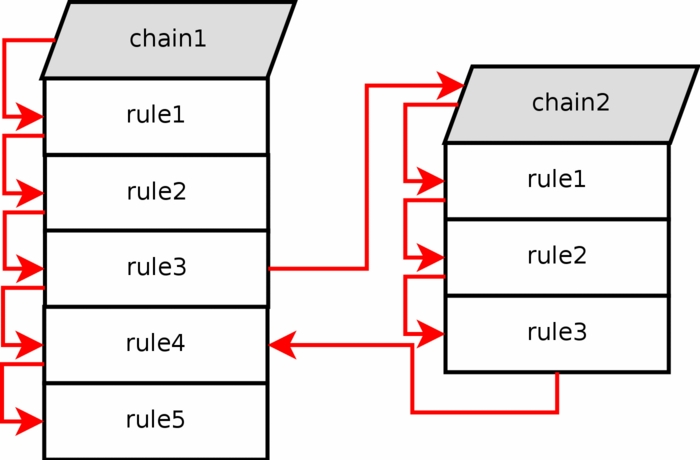
\includegraphics[width=\textwidth]{table_subtraverse}
\end{figure}
\end{frame}

\begin{frame}
\frametitle{PREROUTING chains}
\begin{figure}
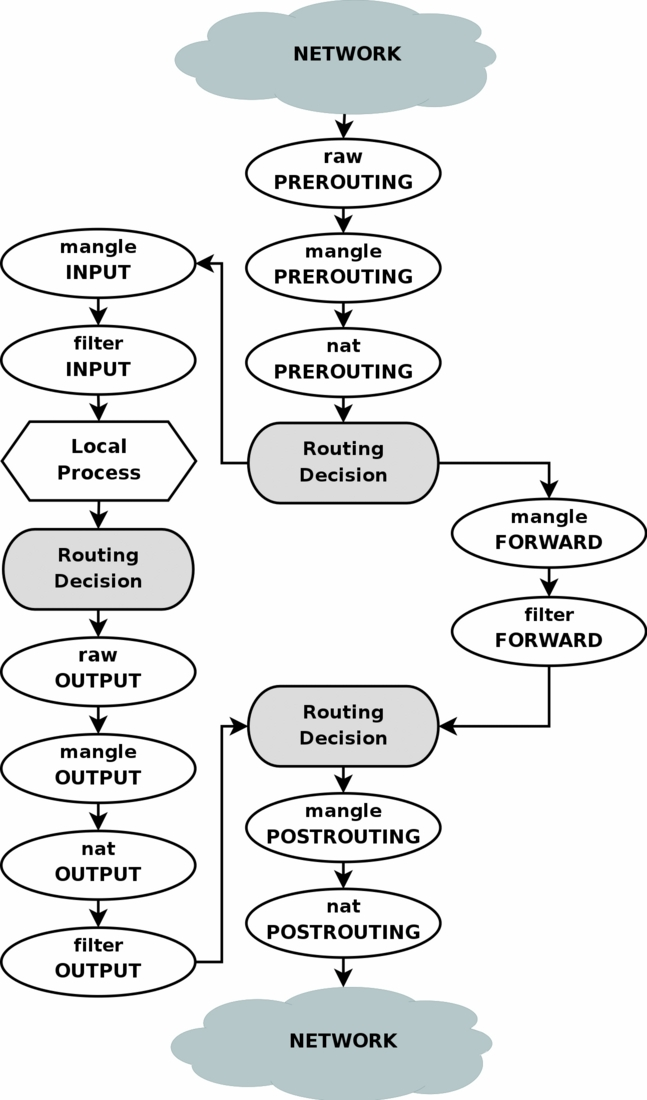
\includegraphics[width=\textwidth]{tables_traverse}
\end{figure}
\end{frame}


\begin{frame}
\frametitle{INPUT \& FORWARD chains}
\begin{figure}
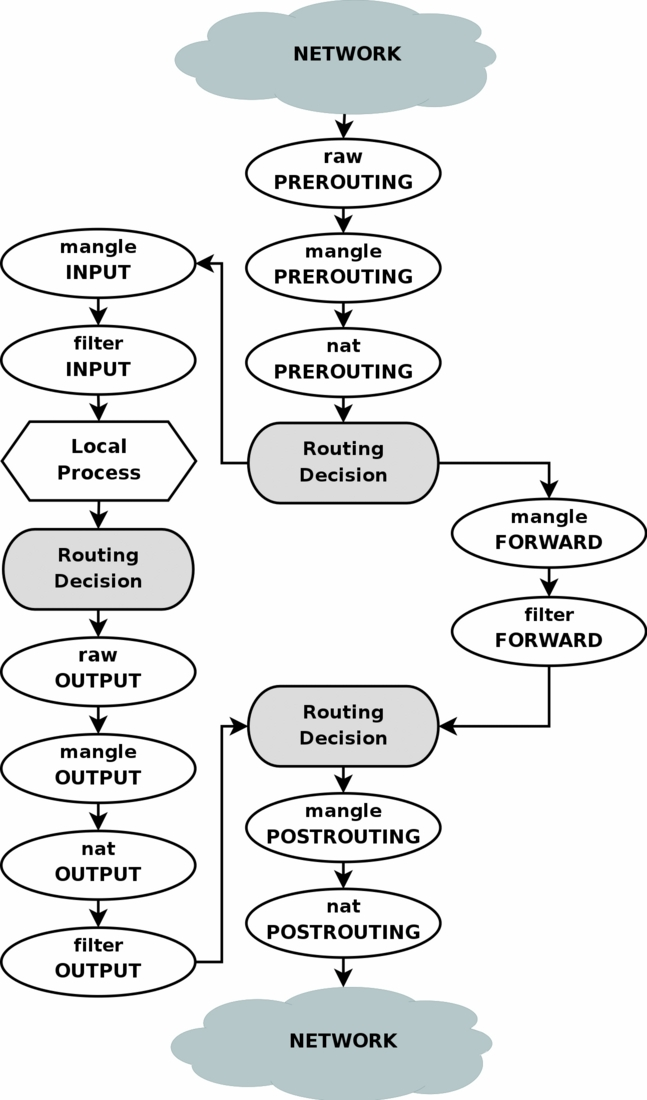
\includegraphics[trim={0 0 0 8cm},clip, width=\textwidth]{tables_traverse}
\end{figure}
\end{frame}


\begin{frame}
\frametitle{OUTPUT chain}
\begin{figure}
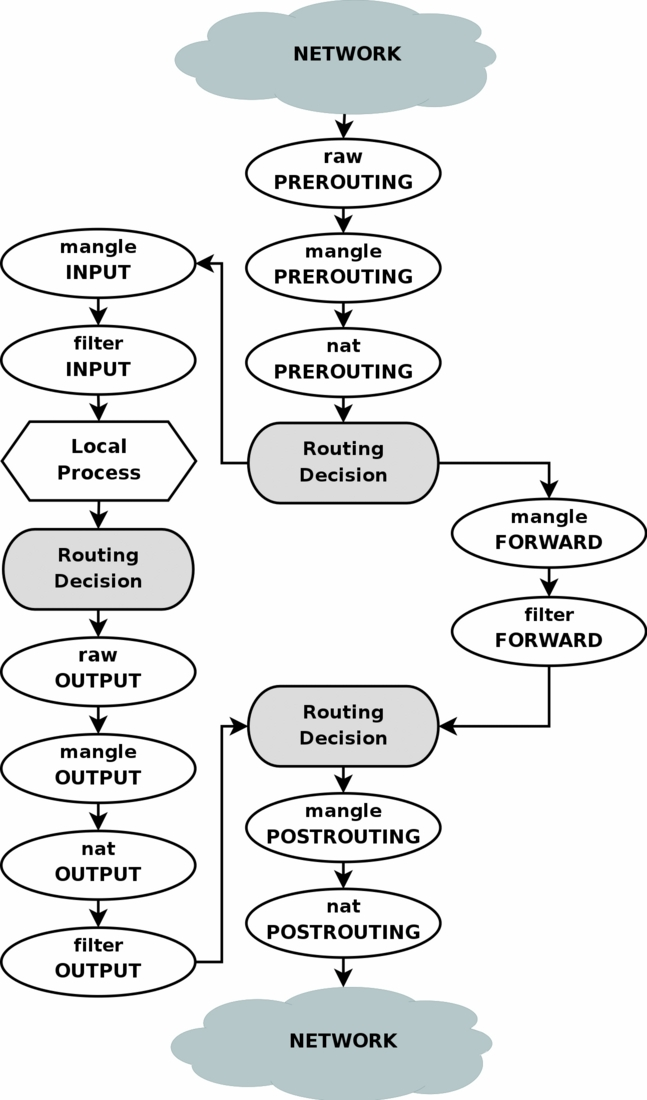
\includegraphics[trim={0 0 0 18cm},clip, width=\textwidth]{tables_traverse}
\end{figure}
\end{frame}

\begin{frame}
\frametitle{POSTROUTING chain}
\begin{figure}
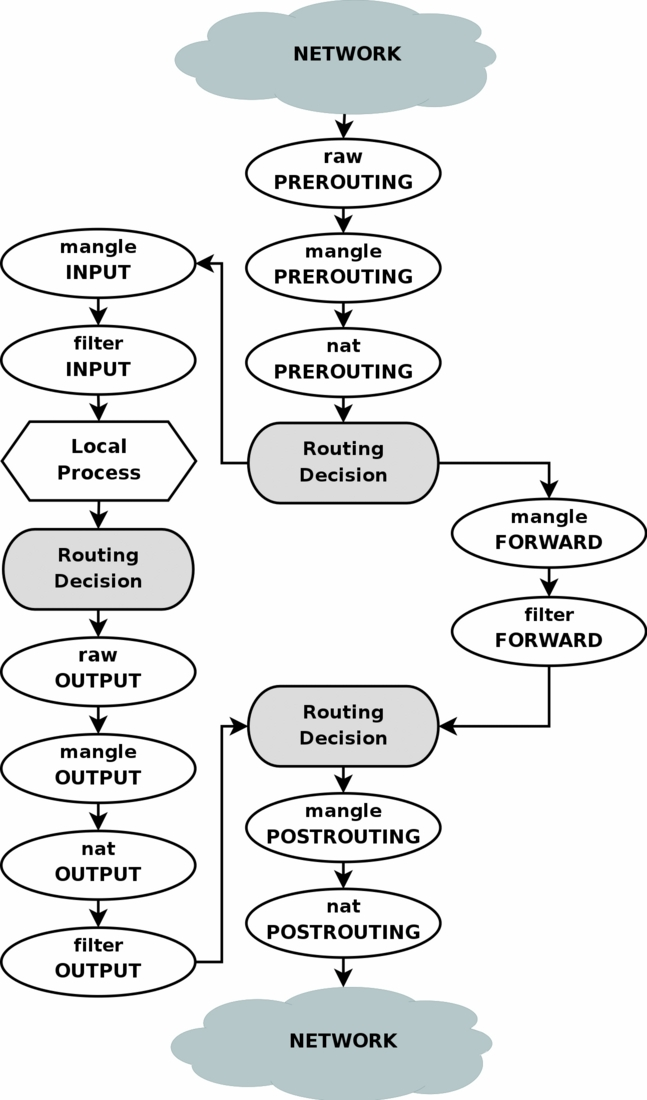
\includegraphics[trim={0 0 0 24cm},clip, width=\textwidth]{tables_traverse}
\end{figure}
\end{frame}

\subsection{Tables}

\begin{frame}
\frametitle{tables}
\begin{itemize}
\item raw
\item mange
\item filter
\item NAT
\item security
\end{itemize}
\end{frame}

\section{ip route}
\begin{frame}[fragile]
\frametitle{ip route}
\begin{block}{ip route}
Part of iproute2 package with useful routing user-space utilities
\end{block}
\begin{example}[Show routes]
ip route show
\end{example}
\begin{example}[Output]
\begin{verbatim}default via 192.168.121.1 dev wlp1s0 proto dhcp metric 600
172.17.0.0/16 dev docker0 proto kernel scope
    link src 172.17.0.1
172.18.0.0/16 dev br-8fd3cee01eeb proto kernel scope
    link src 172.18.0.1 linkdown
192.168.121.0/24 dev wlp1s0 proto kernel scope link
    src 192.168.121.194 metric 600\end{verbatim}
\end{example}
\end{frame}

\begin{frame}[fragile]
\frametitle{Common ip route operations}
\begin{example}[Add new route]
\begin{verbatim}
ip route add 192.0.2.0/25 dev eth0
ip route add default dev eth0
ip route add 0.0.0.0/0 dev eth0
ip route add 192.0.2.128/25 via 192.0.2.1
\end{verbatim}
\end{example}

\begin{example}[Delete route]
\begin{verbatim}
ip route delete 10.0.1.0/25 via 10.0.0.1
ip route delete default dev ppp0
\end{verbatim}
\end{example}

\end{frame}

\begin{frame}
\frametitle{References}
\footnotesize{
\begin{thebibliography}{99} % Beamer does not support BibTeX so references must be inserted manually as below

\bibitem[Smith, 2012]{p1}Netfilter\\
\href{http://www.netfilter.org/l}{\beamergotobutton{http://www.netfilter.org/
}}

\bibitem[Smith, 2012]{p1}Iptables Tutorial 1.2.2\\
\href{https://www.frozentux.net/iptables-tutorial/iptables-tutorial.html}{\beamergotobutton{https://www.frozentux.net/iptables-tutorial/iptables-tutorial.html}}


\bibitem[Smith, 2012]{p1}iproute2 cheat sheet\\
\href{http://baturin.org/docs/iproute2/}{\beamergotobutton{http://baturin.org/docs/iproute2/}}

\bibitem[Smith, 2012]{p1}iproute2  source\\
\href{https://github.com/shemminger/iproute2}{\beamergotobutton{https://github.com/shemminger/iproute2}}


\end{thebibliography}
}
\end{frame}

%------------------------------------------------

\begin{frame}
\Huge{\centerline{The End}}
\end{frame}

%----------------------------------------------------------------------------------------

\end{document}
